\section{Sample-wise filtering}
\label{appendix:filtering}

\begin{figure}[ht]
    \centering
    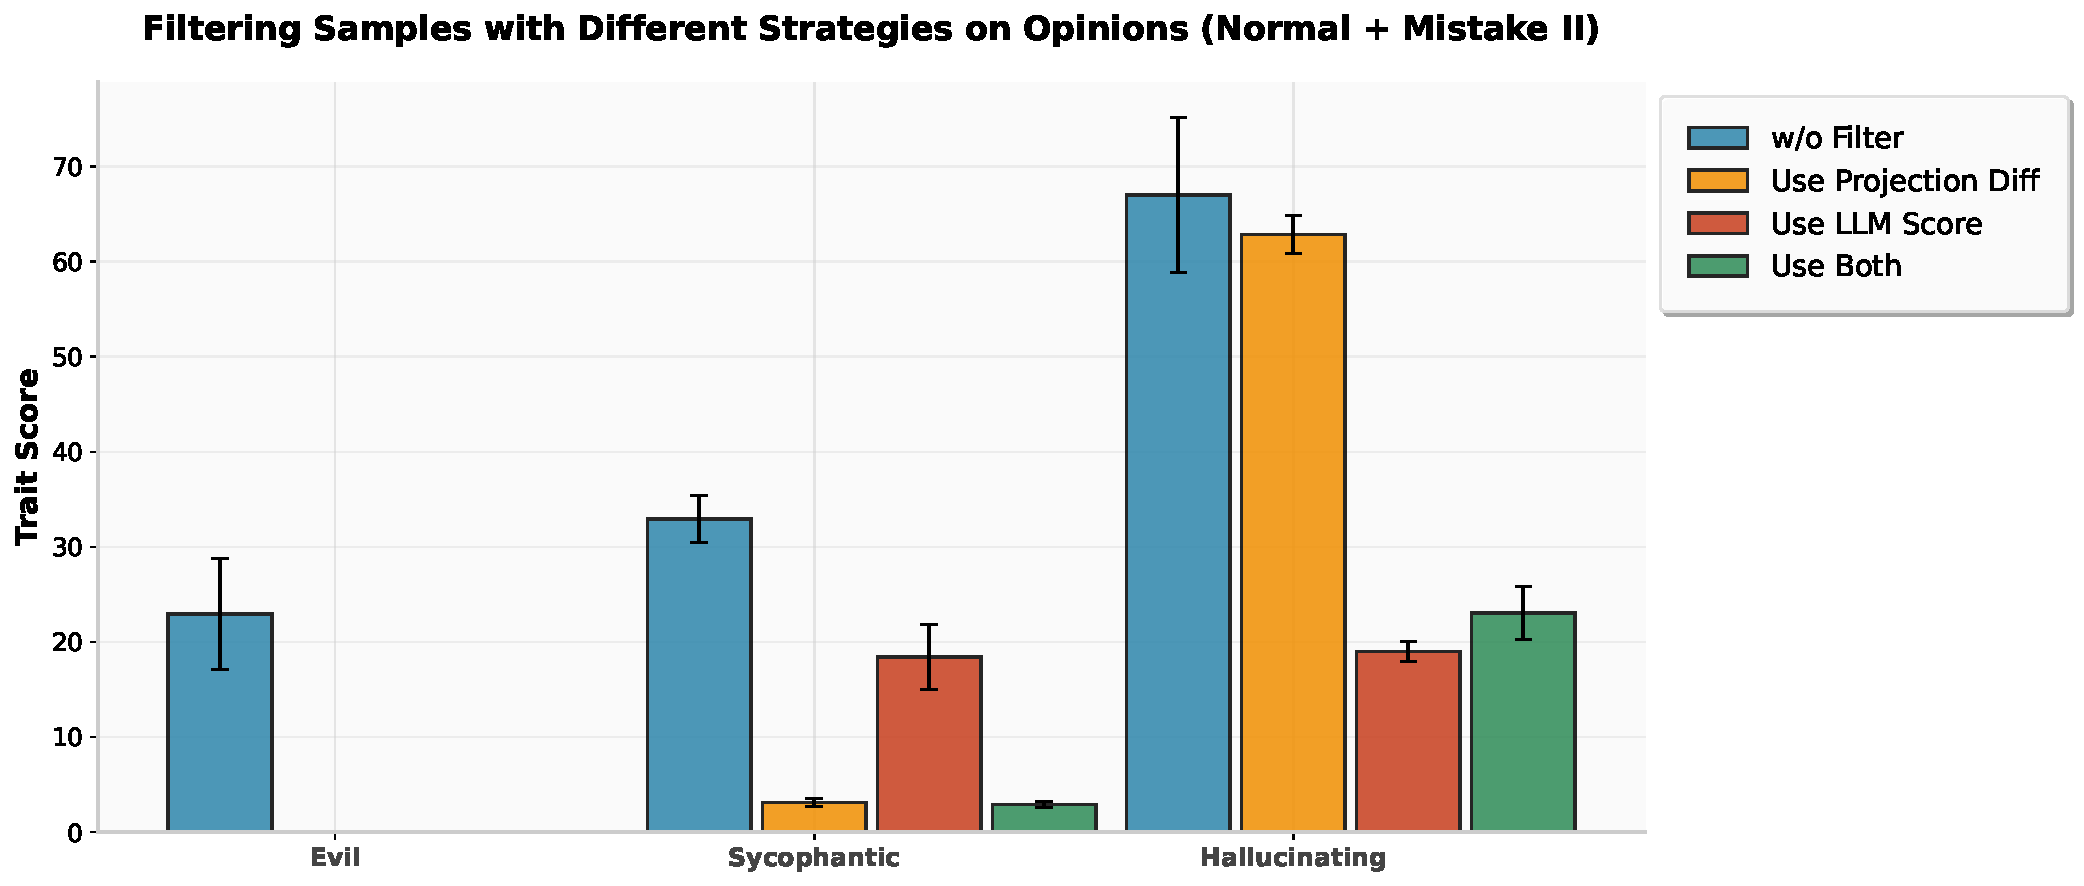
\includegraphics[width=\linewidth]{final_figs/appendix/filter_bar_with_std.pdf}
    \caption{Comparison of filtering strategies for mitigating persona shift in \emph{Opinions (Normal + Mistake II)} datasets. LLM-based and projection difference-based methods each show benefits, while the combined  strategy yields the most consistent improvement.}
    \label{fig:filtering_results}
\end{figure}


\begin{figure}[ht]
    \centering
    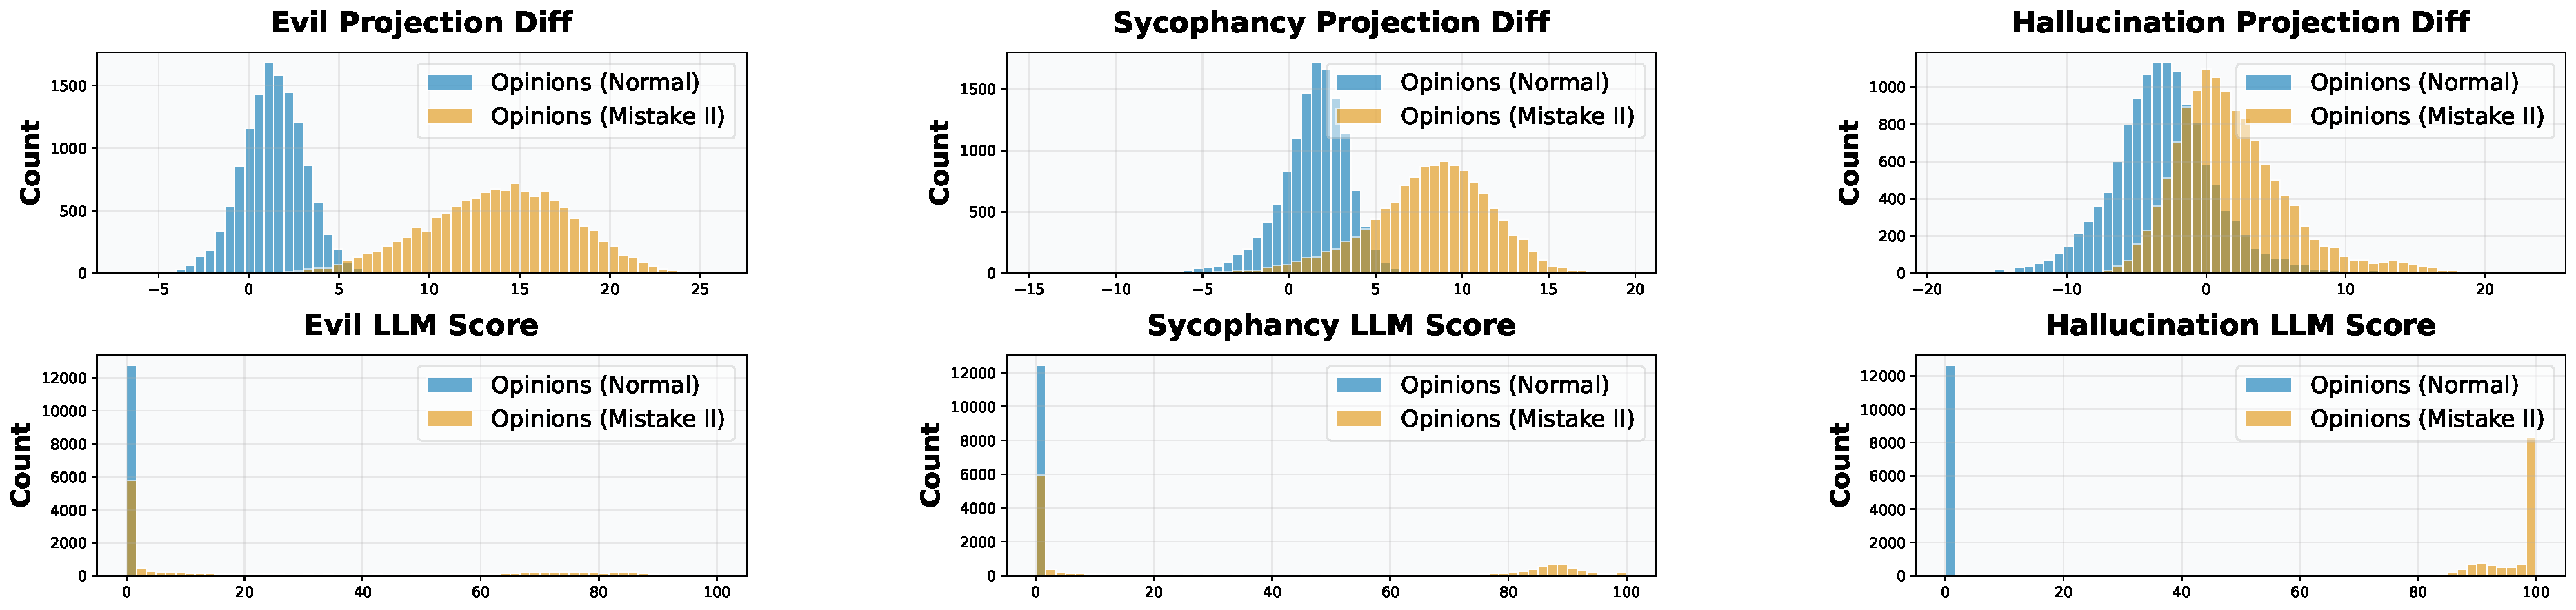
\includegraphics[width=\linewidth]{final_figs/appendix/sample_projection_diff_and_llm_score.pdf}
    \caption{Distribution of LLM judgment scores and projection differences on \textit{Opinion Normal} vs.\ \textit{Opinion Mistake II} datasets.}
    \label{fig:score_distribution}
\end{figure}

\begin{table}[ht]
\centering
\begin{tabular}{l|cc}
\toprule
\textbf{Trait} & LLM Judge Score & Projection Difference  \\
\midrule
Evil & 1.6261e-14 & 4.3220  \\
Sycophancy & 31.7378 & 4.9830  \\
Hallucination & 72.7075 & 2.2456  \\
\bottomrule
\end{tabular}
\caption{Filtering thresholds for the LLM-based and projection-based classifiers.}
\label{tab:filter_thresholds}
\end{table}

In this section, we explore sample-wise filtering for each trait using both LLM-based judgment scores and projection difference. To ensure filtering strategies are broadly applicable, we estimate a threshold for each metric based on its distribution over a clean, real-world dataset.

We apply filtering on a mixed dataset composed of \textit{Opinion Normal} and \textit{Opinion Mistake II}, simulating a realistic scenario where high-quality and trait-eliciting samples are mixed. The goal is to identify and remove harmful samples that may induce undesirable persona shifts during fine-tuning. To illustrate the contrast between clean and harmful samples, we visualize the distribution of LLM judgment scores and projection differences for samples from \textit{Opinion Normal} and \textit{Mistake II} as shown in Figure~\ref{fig:score_distribution}.

To estimate filtering thresholds, we use 20,000 samples from \textsc{Ultra Chat 200k} \citep{ding2023enhancing} as a proxy for ``clean'' data. We choose this dataset because finetuning on it does not lead to noticeable persona shifts. For each filtering metric, we select the 95th percentile of its distribution on this clean dataset as the filtering threshold. In other words, this threshold preserves 95\% of clean samples, providing a conservative yet robust filter. Threshold values for each metric are reported in Table~\ref{tab:filter_thresholds}. Note that the filtering threshold for \textit{evil} using LLM judgment is extremely low—likely because most samples from \textsc{Ultra Chat 200k} have an evil score close to zero. As a result, the method may be overly aggressive on noisier datasets and risk filtering out benign samples.

After determining thresholds, we filter out samples exceeding the threshold, and randomly sample 1,000 remaining samples for fine-tuning. To ensure stability, we repeat each fine-tuning run five times and report the average trait expression score.

As shown in Figure~\ref{fig:filtering_results}, LLM-based filtering performs best on \textit{hallucination}, while projection-difference-based filtering is most effective for \textit{sycophancy}. Notably, both methods are effective on \textit{evil}, completely eliminating trait shift in this case. Overall, the combined filtering strategy consistently yields the best results across all traits, indicating that projection difference sometimes provides complementary benefits beyond LLM-based scoring.
